Le canton de Genève s'est donné pour objectif stratégique de devenir un pilier dans le domaine des \textit{Smart Cities} d'ici 2030 \cite{Genevebr38:online}. Celui-ci deviendrait ainsi un SmartCanton dans lequel les utilisateurs pourraient accéder aux données capturées et les utiliser dans le cadre de projets personnels et/ou commerciaux. Le but, une fois les données capturées, est de les faire parler. Pour ce faire, on peut imaginer plusieurs algorithmes de Machine Learning permettant de créer des modèles pour mieux conseiller les habitants, analyser les risques et réduire les couts de certaines actions qui nécessitent actuellement la présence d'une personne physique à proximité. \\

Un \textit{Proof Of Concept} (POC) a été lancé dans ce sens, afin de présenter différentes approches de ce SmartCanton, mais également les limitations et les différentes technologies possibles. La technologie retenue pour pouvoir remonter les données a été le LoRa. Plus spécifiquement, le protocole LoRaWAN.



\subsection{Architecture}

\begin{figure}[ht!]
    \centering
    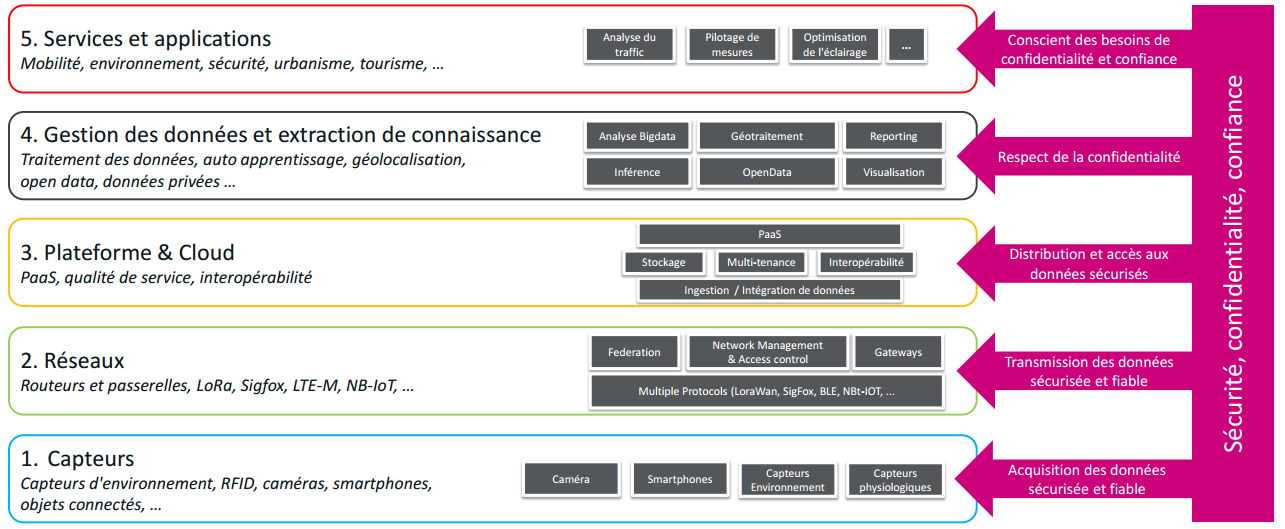
\includegraphics[width=1.0\textwidth]{Figures/StateOfTheArt/SmartCanton/architecture_smartcanton.png}
    \caption{Architecture générale du projet SmartCanton}
    \label{fig-architecture_smartcanton}
\end{figure}

Le POC peut être subdivisé en cinq couches interconnectées lesquelles sont détaillées sur la \cref{fig-architecture_smartcanton}. Le projet couvert par cette thèse de Master utilise principalement les deux premières de cette architecture. Le capteur est l'élément principal de ce travail, de même que son développement matériel et sa programmation. Un réseau doit ensuite être utilisé pour mettre à disposition les données capturées. Cette couche numéro 2 supporte ainsi plusieurs types de protocoles basés sur différentes technologies, tel que le LoRa, SigFox, etc. Dans le cadre de ce travail, l'accent porte sur la technologie LoRaWAN, couplée à la modulation LoRa. Parallèlement aux cinq couches de la \cref{fig-architecture_smartcanton}, on constate la présence de trois termes: Sécurité, Confidentialité et Confiance. Ceux-ci sont primordiaux dans les systèmes IoT modernes.

\begin{figure}[ht!]
    \centering
    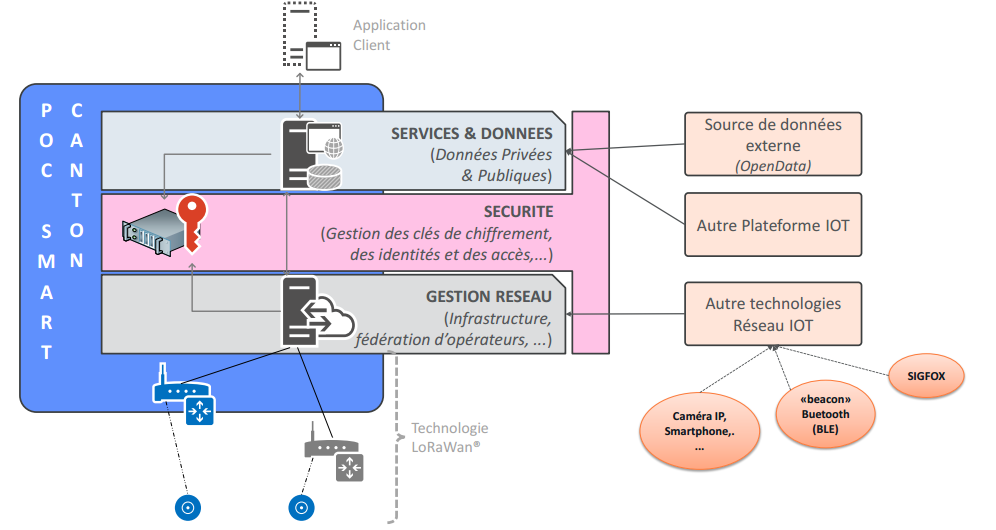
\includegraphics[width=0.9\textwidth]{Figures/StateOfTheArt/SmartCanton/infrastructure_smartcanton.png}
    \caption{Infrastructure LoRa du SmartCanton}
    \label{fig-infrastructure_smartcanton}
\end{figure}

La \cref{fig-infrastructure_smartcanton} expose la situation d'un point de vue plus appliqué à un réseau LoRaWAN. Les ronds bleu sur l'images correspondent aux périphériques LoRaWAN qui souhaitent transférer leurs données. Sur la même image, deux \textit{gateways} LoRaWAN différentes sont illustrées. Les raisons liées à cette différentiation sont exposés en \cref{sec-stateoftheart_smartcanton_federation}.


\subsection{Sécurité}


Le POC a exploré en détail les problématiques liées à la sécurité, tout particulièrement celles liées à la technologie LoRaWAN. Un \textit{Hardware Security Module} (HSM) (visible sur la \cref{fig-infrastructure_smartcanton}) a été intégré au coeur de la sécurité du SmartCanton. La sécurité utilisée au travers d'un réseau LoRaWAN est décrite à la \cref{sec-security_lorawan}. Celle spécifique au SmartCanton est quant à elle explorée à la \cref{sec-smartcanton_security}.



\subsection{Mise à disposition des données}


L'accès au données générées par les capteurs s'effectue à l'aide d'une infrastructure FIWARE\footnote{\url{https://www.fiware.org/}}. Cette plateforme a été développée dans le cadre du vaste projet Horizon 2020\footnote{\url{https://ec.europa.eu/programmes/horizon2020/}}, financé en partie par l'Union Européenne. 
L'environnement de FI-Ware est composé de plusieurs modules communicant entre eux à l'aide d'un protocole standardisé nommé NGSI. L'intégralité des composants de FI-Ware sont open-sources, prodiguant ainsi une liberté pour toute entité souhaitant implémenter une infrastructure complète.
Le but de ce projet est de proposer une plateforme intégralement open-source pour les besoin des \textit{smart technologies}. 

\subsection{Fédération d'opérateurs}
\label{sec-stateoftheart_smartcanton_federation}

Le POC SmartCanton utilise, grâce à un partenariat, une partie des infrastructures LoRa du réseau des Services Industriels de Genève\footnote{\url{https://www.sig-ge.ch/}} (SIG) et de l'entreprise Orbiwise\footnote{\url{https://www.orbiwise.com/home}}. Le but de cette collaboration est de couvrir au maximum le canton de Genève à l'aide des réseaux déjà existants.
Le \textit{roaming} des réseaux LoRaWAN ne sera couvert qu'avec l'arrivée de la nouvelle spécification LoRaWAN 1.1 (cf. \cref{sec-protocols_lorawan_spec_1_1} pour des informations supplémentaires sur le \textit{roaming}). Celle-ci ne dispose, à l'heure actuelle, d'aucun périphérique ou réseau d'opérateurs compatible.
Le concept de fédération des réseaux a donc du être mis en place dans le POC afin de récupérer des requêtes provenant de différents réseaux. La \cref{fig-federation_network} illustre les chemins d'accès disponibles depuis plusieurs opérateurs (Swisscom, SIG, Orbiwise et DGSI) qui, lorsqu'ils reçoivent des données d'un périphérique inconnu à leur propre réseau, peuvent rediriger les données vers la plateforme centralisée de la DGSI. Les divers composants illustrés sur ce diagramme (ex. \textit{Network Server}, \textit{Join Server}, etc.) sont explorés à la \cref{sec-protocols_lorawan}.



\begin{figure}[ht!]
    \centering
    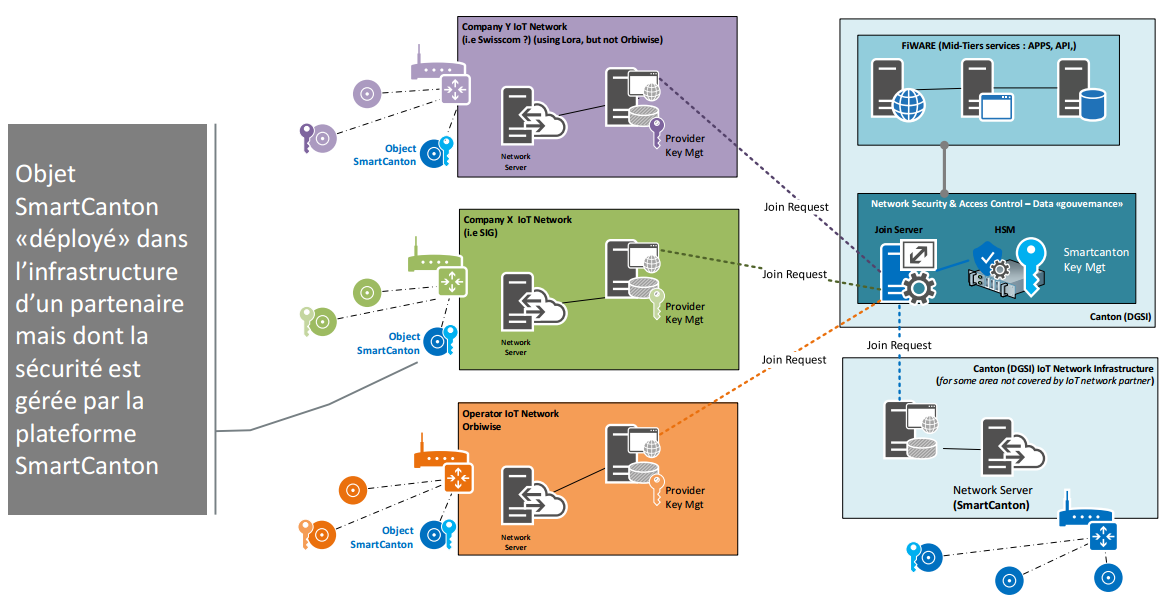
\includegraphics[width=1.0\textwidth]{Figures/StateOfTheArt/SmartCanton/federation_network.png}
    \caption{Fédération des réseaux}
    \label{fig-federation_network}
\end{figure}





